\documentclass[12pt]{article}
\usepackage{graphicx}
\usepackage[ngerman]{babel}
\usepackage[utf8]{inputenc}
\usepackage[T1]{fontenc}
\usepackage{lastpage}
\RequirePackage{subfiles}
\usepackage[a4paper, left=23mm, top=32.5mm, right=25mm, bottom=20mm, headheight=50mm]{geometry}
\usepackage{fancyhdr}
\usepackage{float}
\restylefloat{table}


% my cheaty way of making linebreaks in tables
\usepackage{makecell}
\renewcommand{\cellalign}{tl}
\renewcommand{\theadalign}{tl}

\addto\captionsngerman{
    \renewcommand{\figurename}{Abb.}
}
\renewcommand{\familydefault}{cmss}

% Remove indent
\setlength{\parindent}{0pt}
\setlength{\parindent}{0mm}
\setlength{\parskip}{2mm}

% Header and Footer settings
\pagestyle{fancy}
\fancyhead[L,L] {
\includegraphics[height=10mm]{img/HSLU_Logo.png}}
\fancyhead[R,R] {<projectLogo>}
\fancyfoot[L, L] {PREN 1}
\fancyfoot[C] {\thepage /\pageref{LastPage}}
\fancyfoot[R, R] {\today}
\renewcommand{\headrulewidth}{0pt}
\renewcommand{\footrulewidth}{0.4pt}

% References
\RequirePackage{wrapfig}
\RequirePackage[backend=bibtex]{biblatex}
  \addbibresource{references.bib}

\RequirePackage[linktoc=all]{hyperref}
\hypersetup{
  colorlinks,
  citecolor=black,
  filecolor=black,
  linkcolor=black,
  urlcolor=black
}

% Glossary
\RequirePackage[section, acronym]{glossaries}
    \makeglossaries
    % Override the mark (because the glossary is only a section use the chapter mark)
% else, the \leftmark whould not be the chapter name
\makeatletter
  \renewcommand{\glossarymark}[1]{}
\makeatother

\RequirePackage{nomencl}

\newglossarystyle{acronymindent}{
  \setglossarystyle{long}

  % glossary group skipp
  \renewcommand*{\glsgroupskip}{\vspace{3mm}}
  \renewenvironment{theglossary}
  {
    % bold name
    % \renewcommand{\glsnamefont}[1]{\textbf{#1}}
    \begin{longtable}[l]{@{}p{\dimexpr 1.6cm-\tabcolsep}p{0.8\hsize}}
  }
  {
    \end{longtable}
  }
}

% Make the name bold
\renewcommand{\glsnamefont}[1]{\textbf{#1}}

\newcommand\addglossary{

  \printnomenclature[2cm]
  % Akronyme
  \addcontentsline{toc}
    {section}
    {Akronyme}


  \printglossary[
    title=Akronyme,
    style=acronymindent,
    type=\acronymtype
  ]

  \newpage

}

% Actual document
\title{Produktentwicklung 1}
\author{
\begin{tabular}{ l l l}
  \textbf{Gruppe 4} && \\
  Kasper Jonah & jonah.kasper@stud.hslu.ch & Elektrotechnik\\
  Meyer Alina & alina.meyer@stud.hslu.ch & Informatik \\
  Mumenthaler Marc & marc.mumenthaler@stud.hslu.ch & Maschinentechnik\\
  Schmid Lukas & lukas.schmid@stud.hslu.ch & Informatik\\
  von Atzigen Elias & elias.vonatzigen@stud.hslu.ch & Maschinentechnik \\
  Zimmermann Ivan & ivan.zimmermann@stud.hslu.ch & Elektrotechnik \\
  \\
  \textbf{Betreuender Dozent} && \\
  Thalmann Markus & markus.thalmann@hslu.ch & Elektrotechnik \\
  \\
  \\
  \\
  TA.BA\_PREN1.H2401 &&\\
\end{tabular}
}
\date{\today}

\begin{document}

    \maketitle
    \newpage

    \tableofcontents\thispagestyle{fancy}
    \newpage
    \listoffigures\thispagestyle{fancy}
    \newpage
    \listoftables
    \newpage
      \subfile{glossary.tex}

%%%%%%%%%%%%%%%%%%%%%%%%%%%%%%%%%%%%%%%%%%%%%%%%%%%%%%%%%%%%%%%%%%%%%%%%%%%%%%%%%%%%%%%%%%
%%%%%%%%%%%%%%%%%%%%%%%%%% Add your file here %%%%%%%%%%%%%%%%%%%%%%%%%%%%%%%%%%%%%%%%%%%%
%%%%%%%%%%%%%%%%%%%%%%%%%%%%%%%%%%%%%%%%%%%%%%%%%%%%%%%%%%%%%%%%%%%%%%%%%%%%%%%%%%%%%%%%%%

    % Include files
    \section{Einleitung}

In dieser Dokumenation wird im Rahmen von \acrfull{pren1} die Entwicklung eines autonomen Roboters geplant. Dieser Roboter soll in der Lage sein, ein Wegenetzwerk zu erkennen und diesem zu folgen. Auf den einzelnen Wegen können sich Hindernisse befinden. Die eine Art der Hindernisse sind Pillonen. Wenn sich diese auf einem Pfad befinden, kann dieser nicht befahren werden. Die andere Art der Hindernisse können entfernt werden. Damit der Pfad befahrbar ist, müssen diese jedoch wieder an der selben Stelle zurückgestellt werden.
Das Projekt wird in einem interdiszipilinären Team durchgeführt. Das Team besteht aus Studenten aus den Studiengängen Maschinentechnik, Elektrotechnik und Informatik. Dadurch sind die Kompetenzen, die benötigt werden für die Planung und die Umsetzung des Projektes vorhanden.

In diesem Bericht werden sowohl die Vorgehensweise, als auch die gesamte Planung des Projektes beschrieben. In der Planung wird beschrieben wie das geplante Gesamkonzept erarbeitet wurde. Als erstes wurde eine Technologierecherche durchgeführt. Die einzelnen Lösungen wurden evaluiert und kombiniert. Folgend wurden die Lösungskombinationen evaluiert, woraus sich das Konzept ergab.

Diese Planung bildet die Vorbereitung fuer \acrfull{pren2}. In \acrshort{pren2} wird der geplante Roboter entwickelt. Das Modul wird mit einem Wettbewerb abgeschlossen, wobei die einzelne Gruppen ihre Roboter gegeneinander antreten lassen.

Bei der Konzeptentwicklung des Roboters war es das Ziel einen möglichst simplen Roboter zu bauen, der funktioniert. Der Fokus liegt nicht darauf den schnellsten Roboter zu haben, er sollte jedoch effizient sein.
    \subsection{Aufgabenstellung}

Die Aufgabenstellung ist auf folgender Grafik skizziert. Zentral sind die variablen Bedingungen im Wegenetz. Die Strecke kann durch Pylonen gesperrte Knoten haben. Linien können komplett entfernt sein.  Auf einer Verbindungslinie kann sich ein Hindernis befinden, welches vom Roboter angehoben werden darf. Der Roboter muss danach das Hindernis an die ursprüngliche Stelle zurückstellen. Erreicht der Roboter das Ziel, muss es dies signalisieren.

\begin{figure}[H]
\centering
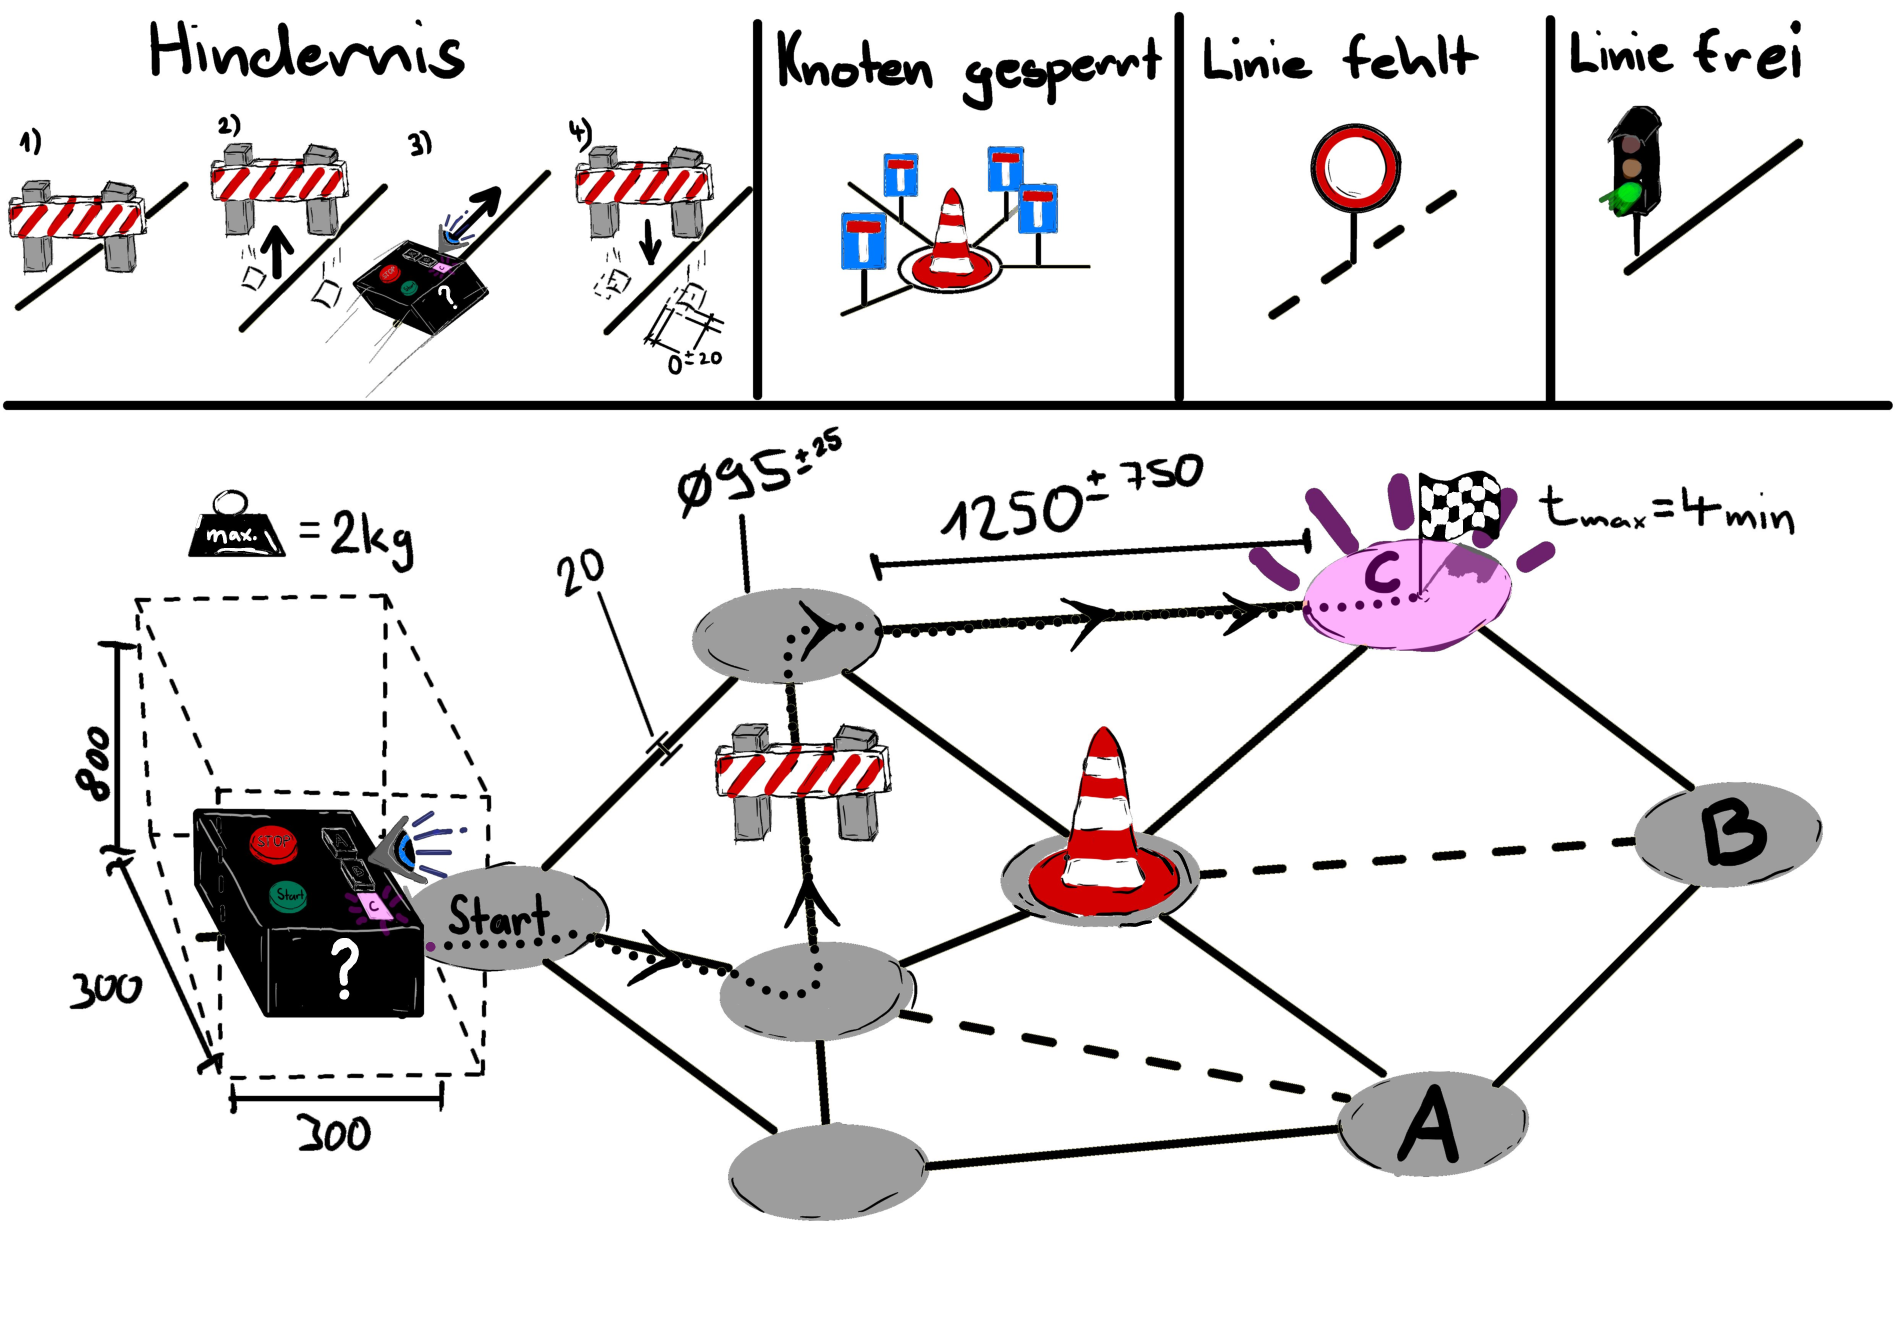
\includegraphics[width=\textwidth]{img/Skizze_Aufgabenstellung_v4.2.png}
\caption{Aufgabenstellung}
\label{fig:aufgebanstellung}
\end{figure}

\subsection{Anforderungsliste}

Die Anforderungsliste wurde basierend auf der Aufgabenstellung erstellt und anschliessend von dem betreuenden Dozenten freigegeben. Zur Strukturierung wurden die Anforderungen in sieben Gruppen gegliedert: Gerät, Sicherheit, Software, Nachhaltigkeit, Demonstration, Wegenetz und Budget. Die einzelnen Anforderungen wurden in die Kategorien Fest-, Mindest-- und Wunschanforderungen unterteilt. Zu jeder Anforderung wurde mindestens eine Fachrichtung definiert, welche für die Einhaltung der
Anforderung verantwortlich ist.

Die vollständige Anforderungsliste befindet sich im Anhang im Kapitel \nameref{anforderungliste}.
    \section{Vorgehen}

Die Vorgehensweise orientiert sich an Scrum, wird jedoch angepasst auf dieses Projekt.
Scrum ist eine agile, inkrementelle Projektmethode, die oft in Softwareentwicklung verwendet wird. Dabei wird in Zeitboxen, die Sprint genannt werden, gearbeitet. Pro Sprint gibt es mehrere Tasks, die bearbeitet werden sollen, sowie Sprintziele. Dies wird in diesem Projekt so gemacht.\cite{wikipedia-scrum}

Normalerweise gibt es tägliche Synchronisationsmeetings. Hier werden diese wöchentlich durchgeführt, ansonsten wird eher asynchron gearbeitet.

Sprintreviews werden durchgeführt im Rahmen der Besprechung der Testatabgaben mit dem Coach. Retrospektiven werden nicht strukturiert durchgeführt, jedoch wird zu Ende jedes Sprints besprochen, ob die Arbeitsweise angepasst werden soll für den nächsten Sprint.

Als Scrum Board wird Microsoft Teams verwendet. Der Backlog wird zu Beginn der Projektes definiert und in einzelne Sprintbacklogs aufgeteilt.

\subsection{Projektorganisation}

Da es sich um eine interdisziplinarische Produktentwicklung handelt, wurde das Team aus jeweils zwei Studierenden aus den Studiengängen \acrfull{elektrotechnik}, \acrfull{informatik} und \acrfull{maschinentechnik} zusammengeführt. In Abbildung \ref{fig:Organigramm} ist die Projektorganisation ersichtlich. 

Im Team wurde Alina Meyer als Projektleiterin gewählt. Zudem benötigt es für die mechanischen und elektrischen Werkstätten in der Hochschule Luzern jeweils eine zuständige Person im Team. Diese wurden Ivan Zimmerman (\acrshort{elektrotechnik}) und Elias von Atzigen (\acrshort{maschinentechnik}) zugeteilt.

Die klare Aufteilung der Rollen ermöglicht es dem Team effizient und zielgerichtet an der Entwicklung des Projekts zu arbeiten. Durch diese Struktur wird gewährleistet, dass jede technische Disziplin angemessen abgedeckt ist und die Kommunikation innerhalb des Teams reibungslos funktioniert.

\begin{figure}[H]
\centering
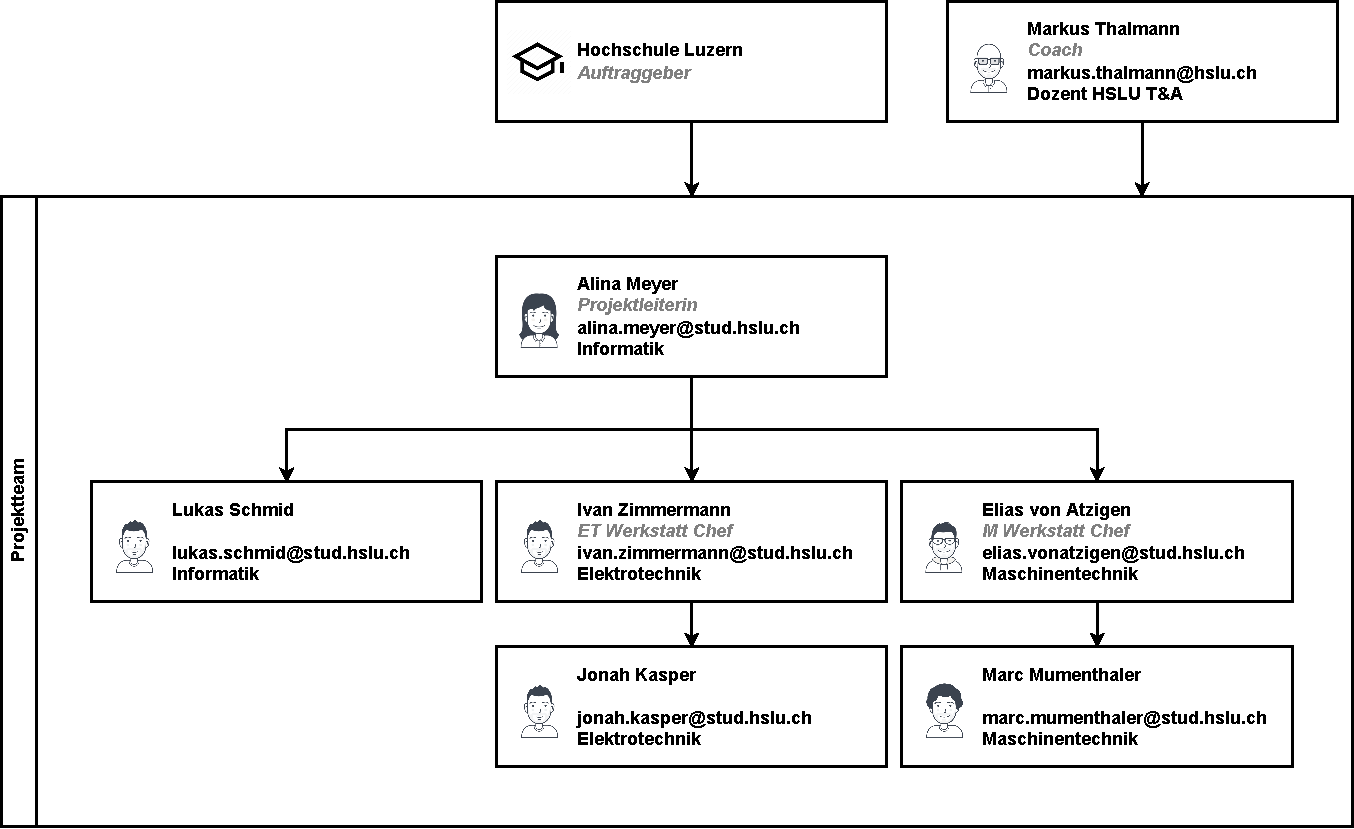
\includegraphics[width=\textwidth]{img/Projektorganisation.pdf}
\caption{Organigramm}
\label{fig:Organigramm}
\end{figure}

\subsection{Datenaustausch}

Zur Zusammenarbeit in diesem Projekt wurde ein Team auf Microsoft Teams erstellt.
Darin ist eine Datenablage, ein Taskboard und ein Chat enthalten. Der Chat wird jedoch weniger verwendet, da die Kommunikation hauptsächlich über WhatsApp erfolgt, damit die Antwortzeiten möglichst kurz sind.

Die Dokumentation wird auf einer eigenen Overleaf Instanz in LaTeX erstellt.

Der erstellte Code wird auf GitHub gespeichert.

Eine detaillierte Auflistung des Datenaustausches und aller Kommunikationsschnittstellen befindet sich im Anhang.

    \section{Projektplanung}

Die Projektplanung wurde anhand der vorgegebenen Abgabetermine durchgeführt.
Da es vier Abgabetermine gibt, wurde das Projekt in vier Sprints aufgeteilt, die jeweils mit einem Meilenstein enden.

\subsection{Risikobewertung}

Die Risiken des Projektes sind gesammelt und bewertet worden das Resultat davon kann der folgenden Grafik entnommen werden.

BILD

Mithilfe von Prototypen sollen so viele Risiken wie möglich, so gut wie möglich vermindert werden. Zum einen wird nach Möglichkeiten gesucht, um das Eintreten zu verhindern, sowie den Schaden bei einem Eintreten zu verkleinern.

\subsection{Projektplan}

Der Projektplan in Tabelle \ref{table:projektplan} zeigt die Meilensteine, die zu erreichen sind.
Die Meilensteine sind die einzelnen Testatabgaben.
Die abzugebenden Dokumente pro Testat bilden die einzelnen Sprintziele.

\begin{table}[h!]
\centering
\begin{tabular}{|l  l l|}
\hline
  \textbf{Meilenstein} & \textbf{Datum} & \textbf{Beschreibung} \\
  \hline
  Meilenstein 1  & 04. Oktober 2024 & \makecell{Projektplan, Skizzierung der Aufgabenstellung,\\ Technologierecherche, Anforderungsliste}\\
  \hline
  Meilenstein 2  & 01. November 2024 & \makecell{Evaluation der Lösungsprinzipien, Auswahl der\\ optimalen Lösungeskombinationen}\\
  \hline
  Meilenstein 3  & 06. Dezember 2024 & \makecell{Freigabe des Gesamtkonzepts, Simulator Wegplanung, \\Dokumentation zu 80\% fertiggstellt}\\
  \hline
  Meilenstein 4  & 10. Januar 2025 & \makecell{Schlussbereicht, Präsentation}\\
  \hline
\end{tabular}
\caption{Projektplan}
\label{table:projektplan}
\end{table}

\subsection{Backlog}

Der Backlog dient als zentrales Planungselement.
In diesem Projekt sind die einzelnen Meilensteine vorgegeben. Aus diesem Grund wurden bereits zu Beginn alle Sprints geplant und der ganze Product Backlog wurde in Sprintbacklogs aufgeteilt. Nach Erreichen eines Meilensteins wird ein Ausblick auf den nächsten Sprint durchgeführt, um allfällige Anpassungen an dem Sprintbacklog vorzunehmen.

\subsection{Sprintplanung}

In den folgenden Kapiteln wurden für jeden Sprint Sprintziele definiert und ein Sprintbacklog erstellt. Für den Sprintbacklog wurden die einzelnen Meilensteine aus dem Projektplan in Epics\footnote{https://www.atlassian.com/agile/project-management/epics} beschrieben. Zu den Epics wurden User Stories erstellt. Der Aufwand der einzelnen Stories wurde mit T-Shirt Grössen geschätzt. Die einzelnen T-Shirt Grössen werden wie folgt in eine Zeitdauer umgerechnet:

\begin{table}[h!]
\centering
\begin{tabularx}\textwidth{|X | X |}
\hline
  \textbf{Grösse} & \textbf{Dauer} \\
  \hline
  S  & 4h - 2d \\
  \hline
  M  & 2d - 5d\\
  \hline
  L  & 5d+\\
  \hline
\end{tabularx}
\caption{T-Shirt Grössen}
\label{table:t-shirt}
\end{table}


\newpage
\subsubsection{Sprint 1: 20. September 2024 - 04. Oktober 2024}

\textbf{Sprintziel:}
\begin{itemize}
    \item Projektplan erstellt
    \item Aufgabenstellung skizziert
    \item Andorderungsliste erstellt
    \item Technologierecherche
\end{itemize}

\textbf{Sprintbacklog:} Der Sprintbacklog von Sprint 1 ist in Tabelle \ref{table:sprint1-backlog} dargestellt.

\begin{table}[H]
\centering
\small
\begin{tabularx}{\textwidth}{|l|l|X|c|}
\hline
  \textbf{Nr.} & \textbf{Titel} & \textbf{Beschreibung} & \textbf{Size}\\
  \hline
  1  & \textbf{Projektorganisation definieren} &&\\
  \hline
  1.1  & Rollendefinition & Die Rollen Projektleiter und Werkstattverwantwortliche werden definiert. & S\\
  \hline
  1.2 & Datenaustausch definieren & Zentrale Datenablage und Kommunikationsschnittstellen definieren.& S\\
  \hline
  1.3 & Ziele definieren & Definieren, wie wir uns den Roboter vorstellen. & S\\
  \hline
  1.4 & Vorgehen definieren & Geeignete Projektmethode wird gewählt. & S\\
  \hline
  2 & \textbf{Aufgabenstellung klären} && \\
  \hline
  2.1 & Anforderungsliste erstellen & Anforderungen, die der Roboter erfüllen muss sammeln& M \\
  \hline
  2.2 & Aufgabenstellung skizzieren & Modellierunge der Aufgabe zum Verständnis. & S \\
  \hline
  3 & \textbf{Projektplanung} && \\
  \hline
  3.1 & Projektplan erstellen & Meilensteine definieren. & S \\
  \hline
  3.2 & Backlog erstellen & Product Backlog für alle Sprints erstellen. & M \\
  \hline
  4 & \textbf{Lösungsvarianten erarbeiten} && \\
  \hline
  4.1 & Teilfunktionen finden & Roboter in Teilfunktionen aufteilen & S \\
  \hline
  4.2 & Technologierecherche & Recherche zu den einzelnen Teilfunktionen  durchführen. & L\\
  \hline
 
\end{tabularx}
\caption{Sprint 1 Backlog}
\label{table:sprint1-backlog}
\end{table}

\newpage
\subsubsection{Sprint 2: 04. Oktober 2024 - 01. November 2024}

\textbf{Sprintziel:}
\begin{itemize}
    \item Evaluation der Lösungsprinzipien
    \item Auswahl der optimalen Lösungeskombinationen
\end{itemize}

\textbf{Sprintbacklog:} Der Sprintbacklog von Sprint 2 ist in Tabelle \ref{table:sprint2-backlog} dargestellt.


\begin{table}[H]
\centering
\small
\begin{tabularx}{\textwidth}{|l|l|X|c|}
\hline
  \textbf{Nr.} & \textbf{Titel} & \textbf{Beschreibung} & \textbf{Size}\\
  \hline
  1  & \textbf{Evaluation Lösungsvarianten} &&\\
  \hline
  1.1  & Workshop Auschlusskriterien & Brainstorming, um herauszufinden, was wir nicht wollen, um Technologien auszuschliessen. & S\\
  \hline
  1.2 & Erste Aussortierung & Lösungsvarianten aussortieren ahhand Auschlusskriterien. & M\\
  \hline
  1.3 & Morphologischer Kasten & Morphologischer Kasten erstellen, um Lösungskombinationen zu ermitteln. & L\\
  \hline
  1.4 & Nutzwertanalyse & Nutzwertanalyse durchführen, um passendste Lösungskombinationen zu ermitteln. & L\\
  \hline
  2 & \textbf{Simulator} && \\
  \hline
  2.1 & Entwicklungsumgebung & Entwicklungsumgebung erstellen. & S \\
  \hline
  2.2 & Konzept erarbeiten & Konzept des Simulators definieren analog zu der Evaluation der anderen Lösungsvarianten. & M \\
  \hline
  2.3 & Wegfindung implementieren & Wegfindung in einem Graphen implementieren. & M \\
  \hline

\end{tabularx}
\caption{Sprint 2 Backlog}
\label{table:sprint2-backlog}
\end{table}

\newpage
\subsubsection{Sprint 3: 01. November 2024 - 06. Dezember 2024}

\textbf{Sprintziel:}
\begin{itemize}
    \item Dokumentation ist zu 80\% fertiggestellt
    \item Simulator ist fertiggstellt
    \item Freigabe des Gesamtkonzepts
\end{itemize}

\textbf{Sprintbacklog:} Der Sprintbacklog von Sprint 2 ist in Tabelle \ref{table:sprint2-backlog} dargestellt.

\begin{table}[H]
\centering
\small
\begin{tabularx}{\textwidth}{|l|l|X|c|}
\hline
  \textbf{Nr.} & \textbf{Titel} & \textbf{Beschreibung} & \textbf{Size}\\
  \hline
  1  & \textbf{Gesamtkonzept} & Gesamtkonzept wird mittels Prototyping ausgearbeitet.&\\
  \hline
  1.1  & Konzept Chassis (M) &  Das Konzept der Form wird definiert. & M\\
  \hline
  1.2  & Konzept Fortbewegung \& Lenkung (M) &  Das Konzept der Fortbewegung wird definiert. & M\\
  \hline
  1.3 & Konzept Hindernisse bewegen (M) & Es wird definiert, wie Hindernisse bewegt werden sollen. & L\\
  \hline
  1.4 & Konzept Linienerkennung (ET) & Die Linienerkennung wird definiert. & M\\
  \hline
  1.5 & Konzept Antriebe (ET) & Der Antrieb und wie dieser angesteuert wird wird definiert. & M\\
  \hline
  1.6 & Konzept Objekterkennung (ET) & Es wird definiert, wie Objekte erkannt werden. & L\\
  \hline
  1.7 & Konzept Steuerung (ET/I) & Es wird definiert, wie der Roboter gesteuert wird. & L\\
  \hline
    1.8 & Konzept Wegfindung (I) & Es wird definiert, wie der Weg, den der Roboter gehen soll, ausgewählt wird.  & M\\
\hline
    1.9 & Konzept Bilderkennung (I) & Es wird definiert, wie das Wegenetzwerk und die Hindernisse erkannt werden. & L\\
\hline
    1.10 & Konzept I/O (M/ET/I) & Es wird definiert, wie das Ziel ausgewählt wird und wie kommuniziert wird, dass der Roboter am Ziel angekommen ist. & M\\
\hline

  2  & \textbf{Simulator} &&\\
  \hline
    2.1 & Hinderniserkennung & Implementieren, dass Hindernisse erkannt und unterschieden werden. Die Reaktion ist je nach Hindernis anders.& M \\
    \hline
  2.2 & Simulator wird fertiggestellt &  Die Entwicklung des Simulators wird abgeschlossen. & M\\
  \hline
  
\end{tabularx}
\caption{Sprint 3 Backlog}
\label{table:sprint3-backlog}
\end{table}

\newpage
\subsubsection{Sprint 4: 06. Dezember 2024 - 10. Januar 2025}

\textbf{Sprintziel:}
\begin{itemize}
    \item Lösung und Gesamkonzept werden präsentiert
    \item Dokumentation wird fertiggestellt und abgegeben
\end{itemize}

\textbf{Sprintbacklog:} Der Sprintbacklog von Sprint 4 ist in Tabelle \ref{table:sprint4-backlog} dargestellt.

\begin{table}[H]
\centering
\small
\begin{tabularx}{\textwidth}{|l|l|X|c|}
\hline
  \textbf{Nr.} & \textbf{Titel} & \textbf{Beschreibung} & \textbf{Size}\\
  \hline
  1  & \textbf{Dokumentation} &&\\
  \hline
  1.1  & Fertigstellung Dokumentation & Die Dokumentation wird fertiggestellt & M\\
  \hline
  2 & \textbf{Präsentation} && \\
  \hline
  2.1 & Präsentation vorbereiten & Gesamtkonzept zusammenfassen. & M \\
  \hline
  2.2 &Präsentation halten & Gesamtkonzept präsentieren. & S \\
  \hline
\end{tabularx}
\caption{Sprint 4 Backlog}
\label{table:sprint4-backlog}
\end{table}


    \section{Technologierecherchen}

\subsection{Mechanik}



\newpage
\subsection{Elektrotechnik}

\subsubsection{Stromversorgung}

\subsubsection{Antriebe}

\begin{table}[H]
\centering
\small
\begin{tabular}{|l|l|l|}
\hline
  \textbf{} & \textbf{Bürstenbehafteter Motor} & \textbf{Bürstenloser Motor (BLDC)}\\
  \hline
  \textbf{Beschreibung}  & \makecell{Einfach und gutes Preis-Leistungsverhältnis} & \makecell{Leichter Motor benötigt jedoch \\zusätzliche Schaltung}\\
  \hline
  \textbf{Vorteile}  & \makecell{-aufgrund linearer Strom-Drehmoment \\Charakteristik gutes Regelverhalten\\-Drehzahleinstellbereich gross} & \makecell{-Belastbar\\-wartungsfrei\\-niedriges Gewicht}\\
  \hline
  \textbf{Nachteile} & \makecell{-schlechte Wärmeableitung\\-Warten von Kommutator und Bürsten}& \makecell{-Sensorsystem notwendig\\-zusätzliche Systemkosten}\\
  \hline
  \textbf{Links} & https://doi.org/10.1007/978-3-658-37423-5& https://doi.org/10.1007/978-3-658-37423-5\\
  \hline
\end{tabular}
\caption{Antriebe}
\label{table:motor1-compare}
\end{table}


\begin{table}[H]
\centering
\small
\begin{tabular}{|l|l|l|}
\hline
  \textbf{} & \textbf{Asynchron Motor} & \textbf{Schrittmotoren}\\
  \hline
  \textbf{Beschreibung}  & \makecell{effizienter Motor} & \makecell{Präziser Motor ohne zusätzliche Steuerung}\\
  \hline
  \textbf{Vorteile}  & \makecell{-robust, wartungsfrei \\-tiefe Herstellungskosten} & \makecell{-wartungsfrei\\-kostengünstig\\-Betrieb ohne weiteren Sensoren}\\
  \hline
  \textbf{Nachteile} & \makecell{-zusätzliche Komponenten nötig für \\Drehzahlverstellung\\-unpräzise ohne Steuerelektronik}& \makecell{-Leistungen müssen bekannt sein\\-niedrige Leistungsdichte}\\
  \hline
  \textbf{Links} & https://doi.org/10.1007/978-3-658-37423-5& https://doi.org/10.1007/978-3-658-37423-5\\
  \hline
\end{tabular}
\caption{Antriebe}
\label{table:motor2-compare}
\end{table}

\subsubsection{Objekterkennung}

\begin{table}[H]
\centering
\small
\begin{tabular}{|l|l|l|}
\hline
  \textbf{} & \textbf{Ultraschall} & \textbf{Optoelektrisch}\\
  \hline
  \textbf{Beschreibung}  & \makecell{Senden und Empfangen von Ultraschall} & \makecell{Senden und Emfpangen von Licht}\\
  \hline
  \textbf{Vorteile}  & \makecell{-geringe Störeinflüsse von Material und Umwelt\\-grosse Reichweite} & \makecell{-Präzise Messungen möglich}\\
  \hline
  \textbf{Nachteile} & \makecell{-Blindzone (min. Reichweite)} & \makecell{-Störeinflüsse von Licht\\-Materialbeschaffenheit}\\
  \hline
  \textbf{Links} & https://doi.org/10.1007/978-3-658-12562-2& doi.org/10.1007/978-3-658-12562-2\\
  \hline
\end{tabular}
\caption{Objekterkennung}
\label{table:et-object-detection-compare}
\end{table}





\newpage
\subsection{Informatik}

\subsubsection{Programmiersprache}

\begin{table}[H]
\centering
\small
\begin{tabularx}{\textwidth}{|l|X|X|}
\hline
\textbf{} & \textbf{Python} & \textbf{Java}\\
  \hline
  \textbf{Beschreibung}  & Interpretierte Programmiersprache & Kompilierte Programmiersprache\\
  \hline
  \textbf{Vorteile}  & \makecell{-Lightweight\\-Beliebt für ML\\-Umfangreiche Bibliotheken\\-Grosser Community Support} & \makecell{-Schnell \\-Möglichkeit für Threading}\\
  \hline
  \textbf{Nachteile} & \makecell{-Langsam} & \makecell{-Heavyweight}\\
  \hline
  \textbf{Links} & https://www.python.org/ & https://www.java.com/en/ \\
  \hline
\end{tabularx}
\caption{Programmiersprachen Vergleich}
\label{table:lang-compare}
\end{table}

\subsubsection{Wegfindung Algorithmus}

Es gibt mehrere Algorithmen, mit denen ein Weg in einem Wegenetzwerk gefunden werden können. Nachfolgend werden einige miteinander verglichen.


\begin{table}[H]
\centering
\small
\begin{tabularx}{\textwidth}{|l|X|X|}
\hline
\textbf{} & \textbf{Dijkstras Algorithmus} & \textbf{A* Algorithmus}\\
  \hline
  \textbf{Beschreibung}  & & \\
  \hline
  \textbf{Vorteile}  & \makecell{} & \makecell{}\\
  \hline
  \textbf{Nachteile} & \makecell{} & \makecell{}\\
  \hline
  \textbf{Links} &  &  \\
  \hline
\end{tabularx}
\caption{Wegfindung Algorithmus Vergleich}
\label{table:path-algo-compare}
\end{table}




\subsubsection{Bilderkennung}

\begin{table}[H]
\centering
\small
\begin{tabularx}{\textwidth}{|l|X|X|}
\hline
\textbf{} & \textbf{Tensorflow} & \textbf{LiteRT} \\
  \hline
  \textbf{Beschreibung}  & TensorFlow ist ein von Google entwickeltes Open-Source-Framework für maschinelles Lernen, das sich durch seine Skalierbarkeit und umfangreichen Bibliotheken auszeichnet. & TensorFlow Lite (LiteRT) ist die abgespeckte Version von TensorFlow, optimiert für die Ausführung auf mobilen und eingebetteten Geräten mit begrenzten Ressourcen. \\
  \hline
  \textbf{Vorteile}  & \makecell{-Gut Dokumentiert\\-Grosse Community\\-Gute Performance} & \makecell{-Optimiert für On-Device ML \\ -Gut Dokumentiert \\ -Gute Performance} \\
  \hline
  \textbf{Nachteile} & \makecell{-Steile Lernkurve \\-Überdimensioniert für einfachere\\ Aufgaben } & \makecell{-Steile Lernkurve} \\
  \hline
  \textbf{Links} & https://www.tensorflow.org & https://ai.google.dev/edge/litert \\
  \hline
\end{tabularx}
\begin{tabularx}{\textwidth}{|l|X|X|}
\hline
\textbf{} & \textbf{PyTorch} & \textbf{OpenCV}\\
  \hline
  \textbf{Beschreibung} & PyTorch ist ein von Facebook entwickeltes Open-Source-Framework für maschinelles Lernen, das für seine dynamischen Berechnungsgraphen und einfache Handhabung bekannt ist. & OpenCV ist eine Open-Source-Bibliothek für Computer Vision, die effiziente Algorithmen für Bild- und Videoverarbeitung bereitstellt. \\
  \hline
  \textbf{Vorteile} & \makecell{-Einfacher zu erlernen als TensorFlow \\ -Unterstützt dynamische Graphen \\ (flexibler bei Modellen) \\ -Stark in Forschung und Experimenten \\ -Grosse Community} & \makecell{-Flache Lernkurve \\ -Grosse Community} \\
  \hline
  \textbf{Nachteile} & \makecell{-Weniger ausgereift für die Produktion \\ im Vergleich zu TensorFlow \\ -Hoher Speicherbedarf} & \makecell{-Rechenintensiv \\ -Schlechte Performance \\ -Nicht die beste Wahl für Deep-Learn-\\ing-Fähigkeiten} \\
  \hline
  \textbf{Links} & https://pytorch.org/ & https://opencv.org/ \\
  \hline
\end{tabularx}
\caption{Vision Objekterkennung Vergleich}
\label{table:vision-object-detection-compare}
\end{table}

\textbf{Bilderkennung Software:} Nachfolgend werden einige Softwarelösungen verglichen mit denen eine Bilderkennung durchgeführt werden könnten.

\vspace{10pt}
\hrule
\textbf{Variante 1: TensorFlow}

Beschreibung:

Vorteile:
\begin{itemize}
    \item Gut Dokumentiert
    \item Grosse Community
    \item Gute Performance dank Hardware Beschleunigung
\end{itemize}


Nachteile:
\begin{itemize}
    \item Internetzugang nötig
    \item Steile Lernkurve
    \item Überdimensioniert für einfacher Aufgaben
\end{itemize}

Links: https://www.tensorflow.org/

\vspace{5pt}
\hrule

\textbf{Variante 1: LiteRT (ehemals: TensorFlow Lite}

Beschreibung:

Vorteile:
\begin{itemize}
    \item Optimiert für On-Device ML Applikationen
    \item Gut Dokumentiert
    \item Grosse Community
    \item Gute Performance dank Hardware Beschleunigung
    \item Kein internetzugang nötig
\end{itemize}


Nachteile:
\begin{itemize}
    \item Steile Lernkurve
    \item Überdimensioniert für einfacher Aufgaben
\end{itemize}

Links: https://www.tensorflow.org/

\vspace{5pt}
\hrule

\textbf{Variante 2: OpenCV}

Beschreibung:

Vorteile:
\begin{itemize}
    \item kein Internetzugang nötig
    \item Leicht zu erlenen und zu implementieren
    \item Grosse Community, viele Tutorials und Beispiele verfügbar.
\end{itemize}

Nachteile:
\begin{itemize}
    \item Rechenintensiv, schlechte Performance (je nach Aufgabe)
    \item Nicht die beste Wahl für Deep-Learning-Fähigkeiten
\end{itemize}
Links: https://opencv.org/



\textbf{Bilderkennung Kamera:} Nachfolgend werden einige Varianten verglichen, die als Kamera verwendet werden könnten.

Muss-Kriterium: Platz auf Raspi

\begin{table}[H]
\centering
\small
\begin{tabularx}{\textwidth}{|l|X|X|}
\hline
\textbf{} & \textbf{Raspberry Camera Modul} & \textbf{USB Webcam}\\
  \hline
  \textbf{Beschreibung} &  & \\
  \hline
  \textbf{Vorteile}  & \makecell{-Kompatibilität mit Raspberry Pi \\ -CSI Konnektor} & \makecell{-Grössere Auswahl an Möglichkeiten \\ -Halterung meist inklusive \\ -Schwenkbar und Drehbar} \\
  \hline
  \textbf{Nachteile} & \makecell{-Kein Gehäuse \\ -Keine Halterung} & \makecell{} \\
  \hline
  \textbf{Links} & https://www.raspberrypi.com/documentation/accessories/camera.html & \\
  \hline
\end{tabularx}
\begin{tabularx}{\textwidth}{|l|X|X|}
\hline
\textbf{} & \textbf{GigE USB Kamera} & \textbf{} \\
  \hline
  \textbf{Beschreibung}  & & \\
  \hline
  \textbf{Vorteile}  & \makecell{} & \makecell{} \\
  \hline
  \textbf{Nachteile} & \makecell{} & \makecell{} \\
  \hline
  \textbf{Links} & & \\
  \hline
\end{tabularx}
\caption{Kamera Vergleich}
\label{table:camera-compare}
\end{table}
    \section{Evaluation Lösungsprinzipien}

Aus der vorhergehenden Technologierecherche wird pro Studiengang ein Morphologischer Kasten erstellt. Dieser wird befüllt mit den Teilfunktionen und den recherchierten Technologien. Damit werden die Lösungsprinzipien evaluiert und verschiedene Varianten werden gefunden. Ein Ueberblick ueber alle Morphologischen Kasten befindet sich im Anhang. TODO LINK

\subsection{Maschinentechnik Morphologischer Kasten}

PLACEHOLDER

\subsection{Elektrotechnik Morphologischer Kasten}

PLACEHOLDER

\subsection{Informatik Morphologischer Kasten}

PLACEHOLDER

\subsection{Simulator Morphologischer Kasten}

Kante entfernen nicht, weil gibt ev keinen Weg mehr, zu risky

Knoten nur markieren nicht noetig, bringt keinen Vorteil


\newpage
\section{Auswahl Lösungskombinationen}

Zur Auswahl der passendsten Lösungskombination wird pro Teilbereich eine Nutzwertanalyse durchgeführt. Die Kriterien und deren Gewichtung sind individuell pro Teilbereich, damit sie ideal passen.

\subsection{Maschinentechnik Nutzwertanalyse}

PLACEHOLDER

\subsection{Elektrotechnik Nutzwertanalyse}

PLACEHOLDER

\subsection{Informatik Nutzwertanalyse}

PLACEHOLDER

\subsection{Simulator Nutzwertanalyse}

PLACEHOLDER

Schnelligkeit vernachlaessigbar weil: nur 8 Knoten und weil macht sehr wenig aus, viel wichtiger ist Lightweight, da nur 1 Raspi in Realitaet und wollen moeglichst realitaetsgetreu das machen

\newpage
\section{Gesamtkonzept}

Aus den morphologischen Kasten und den Nutzwertanalysen wurde folgendes Gesamtkonzept ermittelt. 


    \section{Fazit}

Ausblick: Entwicklungskosten, Aufwand

Lessons Learned


    

\section{Template}
\subsection{Some subsection}
Lorem ipsum dolor sit amet, officia excepteur ex fugiat reprehenderit enim labore culpa sint ad nisi Lorem pariatur mollit ex esse exercitation amet. Nisi anim cupidatat excepteur officia. Reprehenderit nostrud nostrud ipsum Lorem est aliquip amet voluptate voluptate dolor minim nulla est proident. Nostrud officia pariatur ut officia. Sit irure elit esse ea nulla sunt ex occaecat reprehenderit commodo officia dolor Lorem duis laboris cupidatat officia voluptate. Culpa proident adipisicing id nulla nisi laboris ex in Lorem sunt duis officia eiusmod. Aliqua reprehenderit commodo ex non excepteur duis sunt velit enim. Voluptate laboris sint cupidatat ullamco ut ea consectetur et est culpa et culpa duis.

\subsection{Another subsection: Liste}
How to make a bullet-point list.
\begin{itemize}
    \item First item
    \item Second item
    \item Third item
\end{itemize}

 And another one:
 
\begin{itemize}
    \item First item
    \item Second item
\end{itemize}
\subsection{Third subsection: Nummerierte Liste}
How to make a numbered list:
\begin{enumerate}
    \item First enum
    \item Second enum
    \item Third enum
\end{enumerate}
\subsubsection{Some sub-subsection}
Lorem ipsum dolor sit amet, qui minim labore adipisicing minim sint cillum sint consectetur cupidatat.


\subsection{Some subsection: Bild einfuegen}
Lorem ipsum dolor sit amet, officia excepteur ex fugiat reprehenderit enim labore culpa sint ad nisi Lorem pariatur mollit ex esse exercitation amet. Nisi anim cupidatat excepteur officia. Reprehenderit nostrud nostrud ipsum Lorem est aliquip amet voluptate voluptate dolor minim nulla est proident. Nostrud officia pariatur ut officia. Sit irure elit esse ea nulla sunt ex occaecat reprehenderit commodo officia dolor Lorem duis laboris cupidatat officia voluptate. Culpa proident adipisicing id nulla nisi laboris ex in Lorem sunt duis officia eiusmod. Aliqua reprehenderit commodo ex non excepteur duis sunt velit enim. Voluptate laboris sint cupidatat ullamco ut ea consectetur et est culpa et culpa duis.

\begin{figure}[h]
\centering

\includegraphics[width=\textwidth]{img/HSLU_Logo.png}
\caption{Sample caption}
\label{fig:hslu-logo}
\end{figure}

Here we can reference image \ref{fig:hslu-logo} if a label has been defined when inserting the image. If you do this it will be uniform.

\subsubsection{Some sub-subsection: Tabelle}

This is how you make a table and reference it like this: \ref{table:template}:

\begin{table}[h!]
\centering
\begin{tabular}{ |l| l| l|} % Dimension breite
  \textbf{Column Header 1} & \textbf{Column Header 2} &  \textbf{Column Header 3}\\
  \hline
  
  Row 1, Col1 & Row 1, Col 2 & Row 1, Col 3\\

  Row 2 &Row 2 & Row 2 \\
  
  Row 3 & Row 3 & Row 3 \\
  
  
  Only fill first Col && and the last\\
\end{tabular}
\caption{Table to show how to use tables}
\label{table:template}
\end{table}

\subsection{Subsection: Akronyme und Quellen}

For acronym entries, add them to the "glossary.tex" file and reference them like this: \acrfull{pren1} when you use them for the first time.

When you wanna use the short form do this \acrshort{pren1}.

How to use a source\cite{wikipedia-scrum}.

%%%%%%%%%%%%%%%%%%%%%%%%%%%%%%%%%%%%%%%%%%%%%%%%%%%%%%%%%%%%%%%%%%%%%%%%%%%%%%%%%%%%%%%%%%
%%%%%%%%%%%%%%%%%%%%%%%%%%%%%%%%%%%%%%%%%%%%%%%%%%%%%%%%%%%%%%%%%%%%%%%%%%%%%%%%%%%%%%%%%%
%%%%%%%%%%%%%%%%%%%%%%%%%%%%%%%%%%%%%%%%%%%%%%%%%%%%%%%%%%%%%%%%%%%%%%%%%%%%%%%%%%%%%%%%%%


    % TODO Glossary doesn't work yet
    \newpage
    \addglossary

    % Literaturverzeichnis
  \newpage
  \addcontentsline{toc}
    {section}
    {Literatur}
  \printbibliography[
    heading=subbibliography
  ]

  % Anhang
  \addcontentsline{toc}
    {section}
    {Anhang}
  \newpage
\section{Anhang}

\subsection{Anforderungsliste}\label{anforderungliste}
Die erste Version der Anforderungsliste ist nachfolgend angehängt.

\begin{table}[H]
\centering
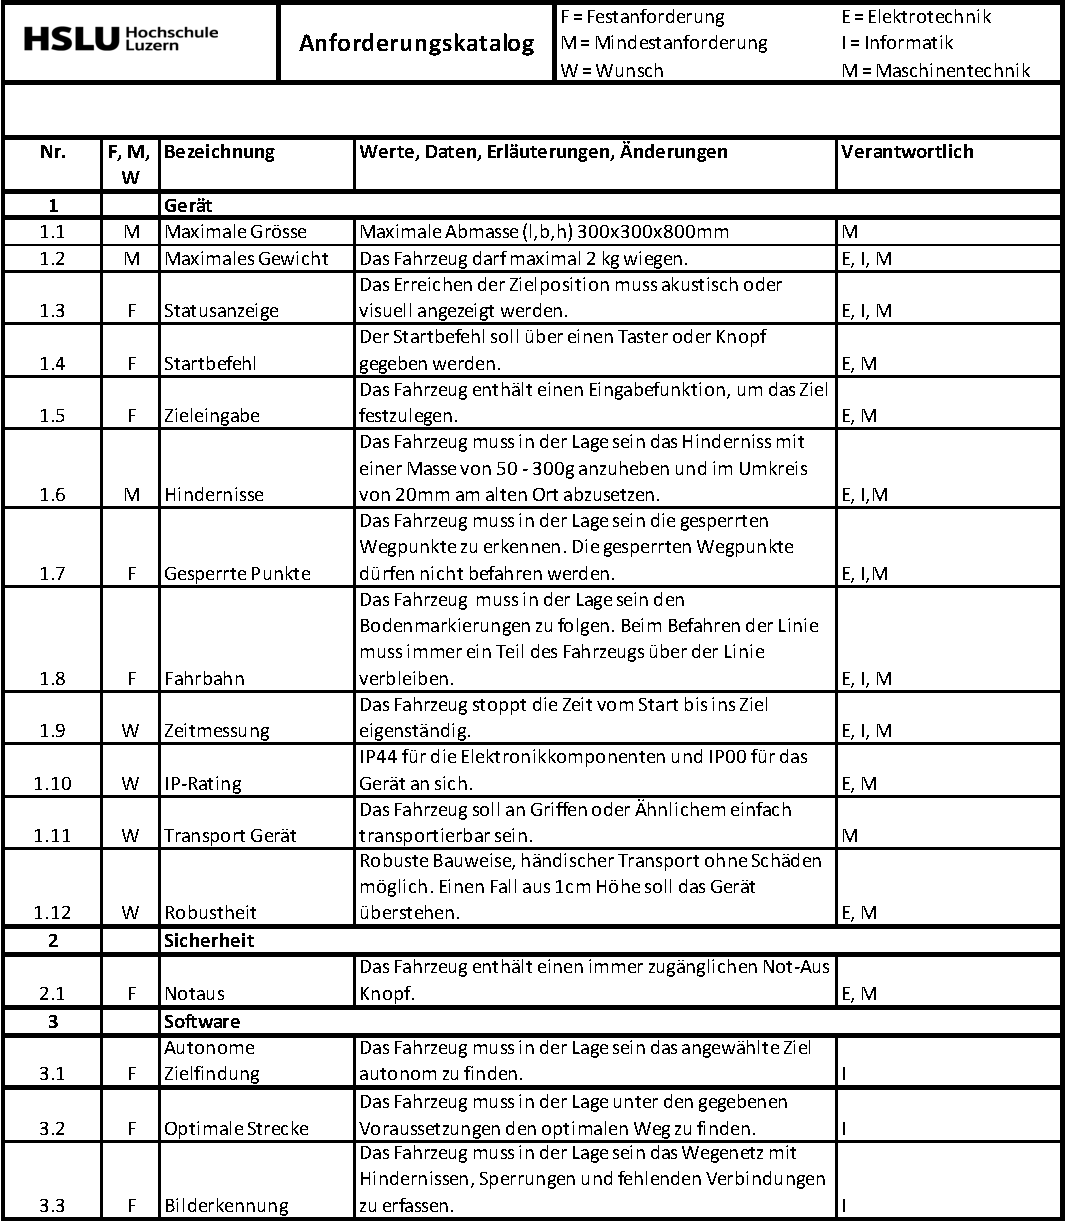
\includegraphics[width=\textwidth]{assets/Anforderungsliste_V1.01_page1.pdf}
\caption{Anforderungsliste Teil 1}
\label{table:anforderungsliste_page1}
\end{table}
\newpage

\begin{table}[H]
\centering
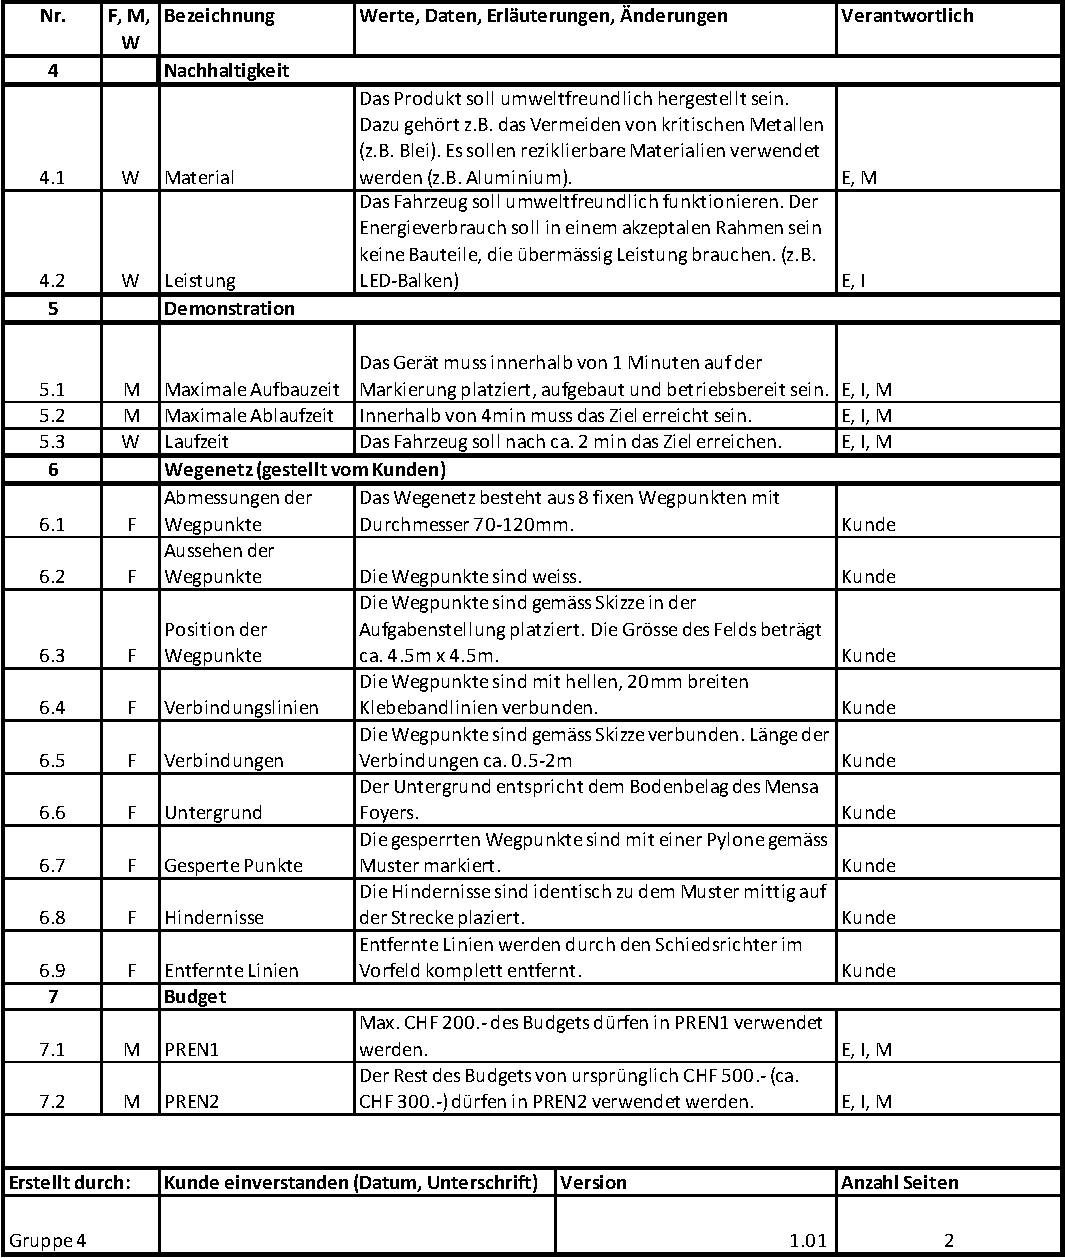
\includegraphics[width=\textwidth]{assets/Anforderungsliste_V1.01_page2.pdf}
\caption{Anforderungsliste Teil 2}
\label{table:anforderungsliste_page2}
\end{table}
\newpage

\begin{landscape}
\subsection{Kommunikationsplan}\label{kommunikationsplan}
Die Kommunikationskanäle sind folgendermassen definiert:

\begin{table}[H]
\centering
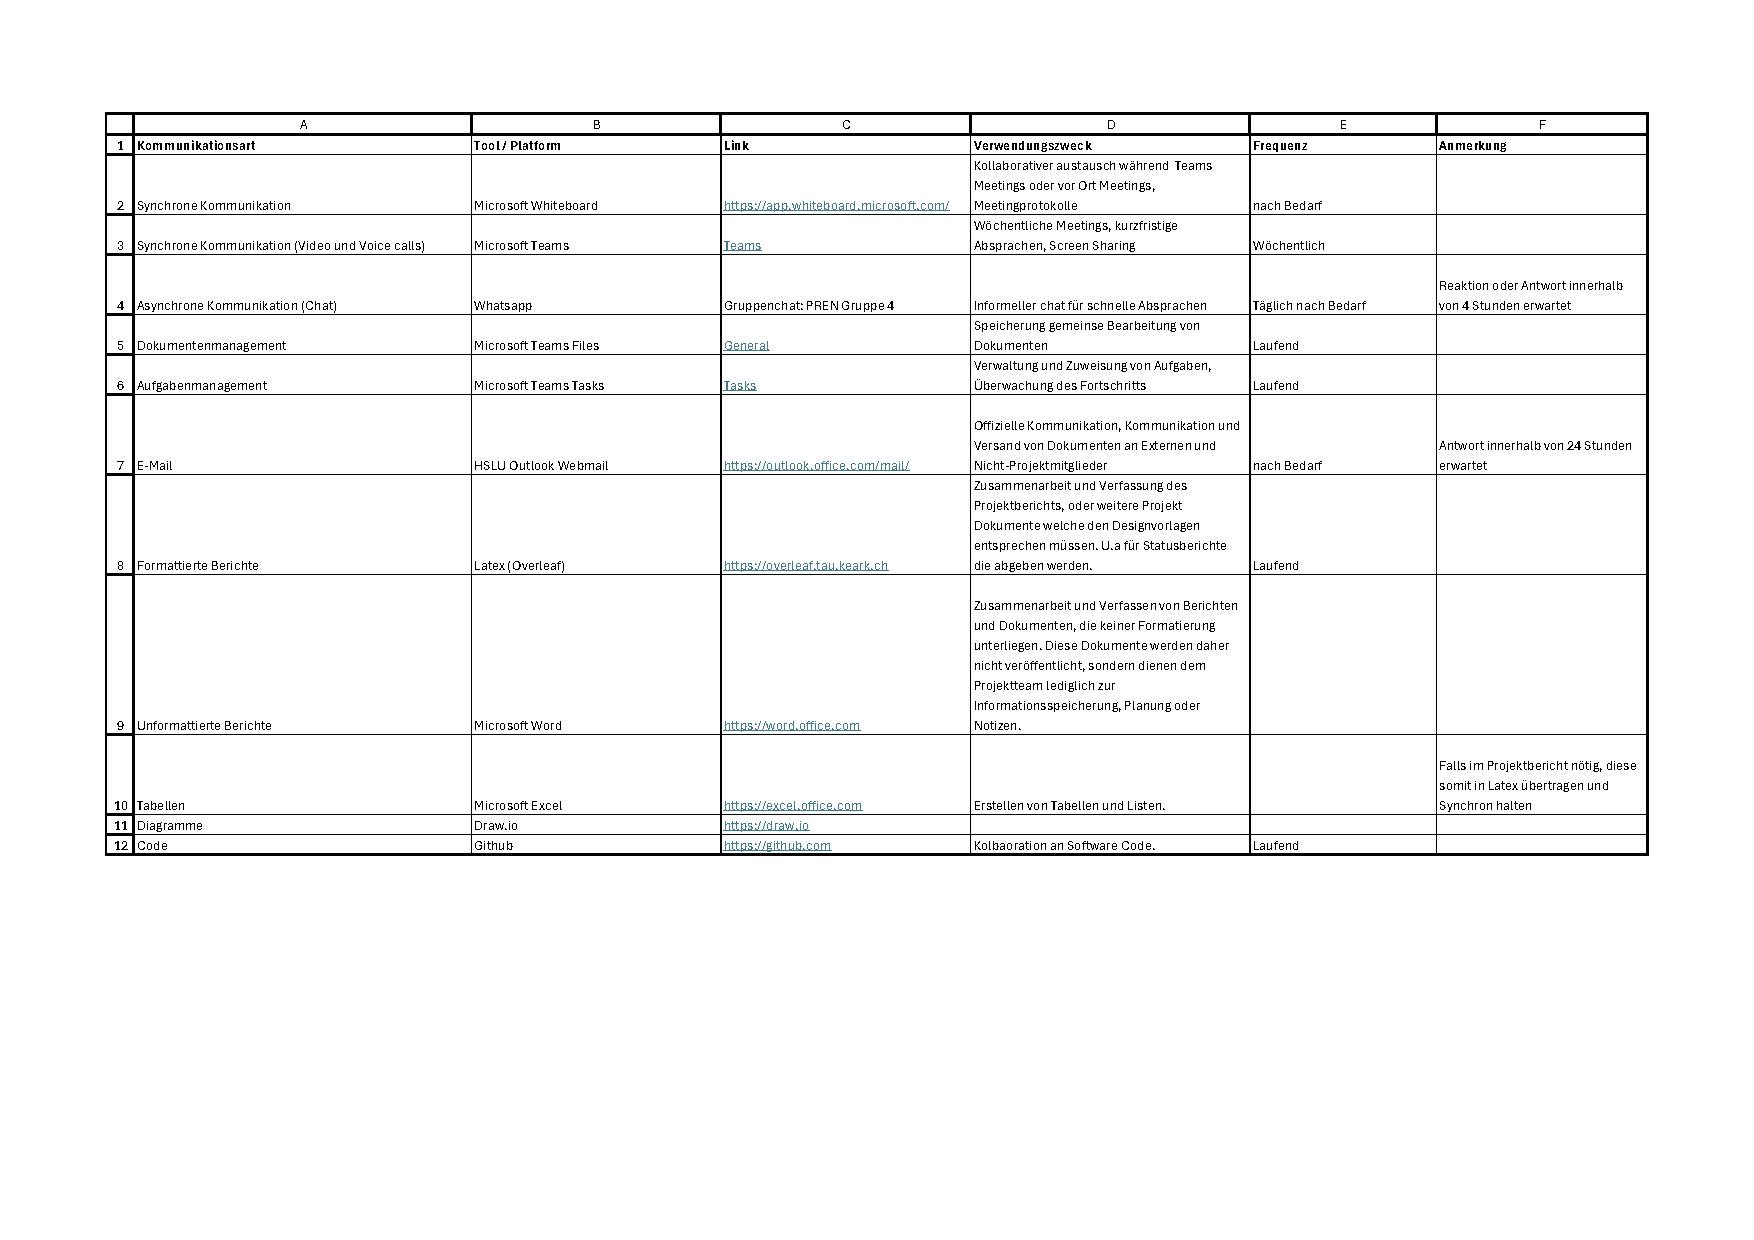
\includegraphics[width=240mm]{assets/Kommunikationschnittstellen.pdf}
\caption{Kommunikationsplan}
\label{table:communications-plan}
\end{table}
\end{landscape}

%%%%%%%%%%%%%%%%%% Technologierecherche %%%%%%%%%%%%%%%%%%%%

\subfile{parts/a-technologierecherchen}


%%%%%%%%%%%%%%%%%%%%%%%%%%%%%%%%%%%%%%%%%%%%%
%%%%%%% Entfernt, weil bereits in Doc   %%%%%
%%%%%%%%%%%%%%%%%%%%%%%%%%%%%%%%%%%%%%%%%%%%%
%\subsection{Morphologischer Kasten}\label{Morphologischer Kasten}
%Nachfolgend die Morphologischen Kästen, unterteilt in die jeweiligen Studiengänge, Elektrotechnik, Informatik und Maschinentechnik. %Jeder Kasten hat 3 Varianten eingezeichnet. Variante A: Gelb, Variante B: Rot, Variante C: Grün.
%
%\begin{table}[H]
%\centering
%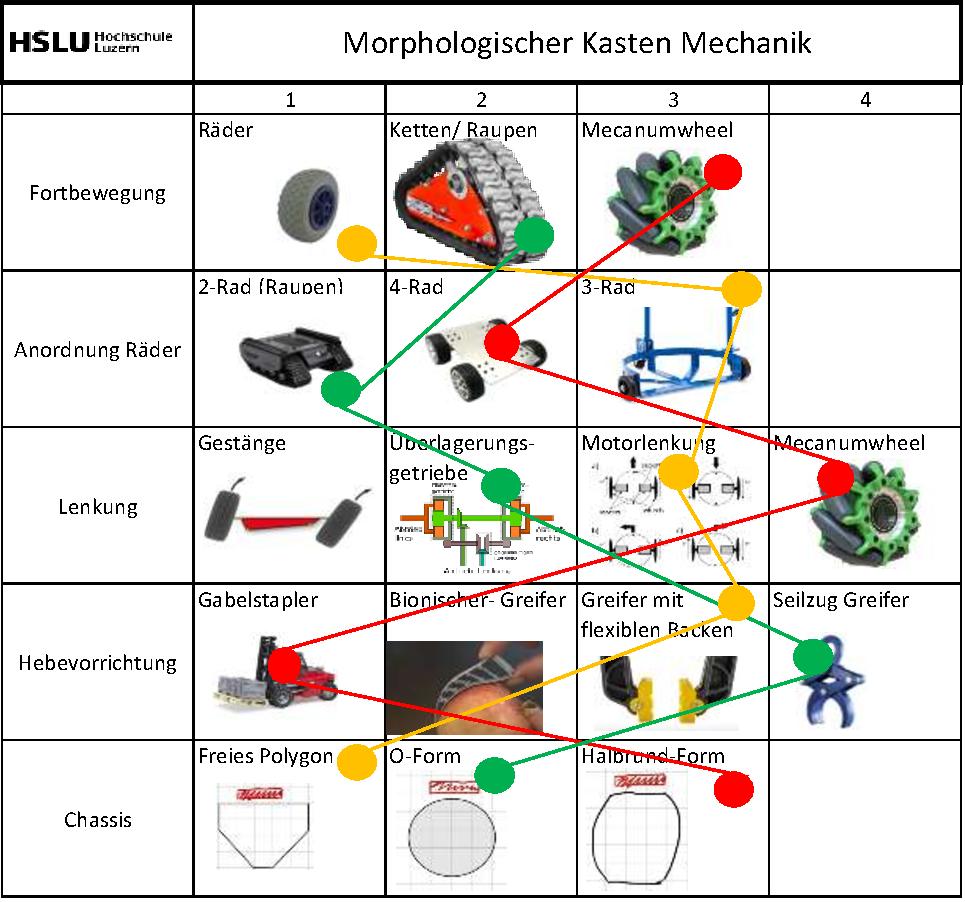
\includegraphics[width=\textwidth]{assets/MK_Maschinentechnik.pdf}
%\caption{Morphologischer Kasten: Maschinentechnik}
%\label{table:MK-Maschinentechnik}
%\end{table}
%\newpage
%\begin{table}[H]
%\centering
%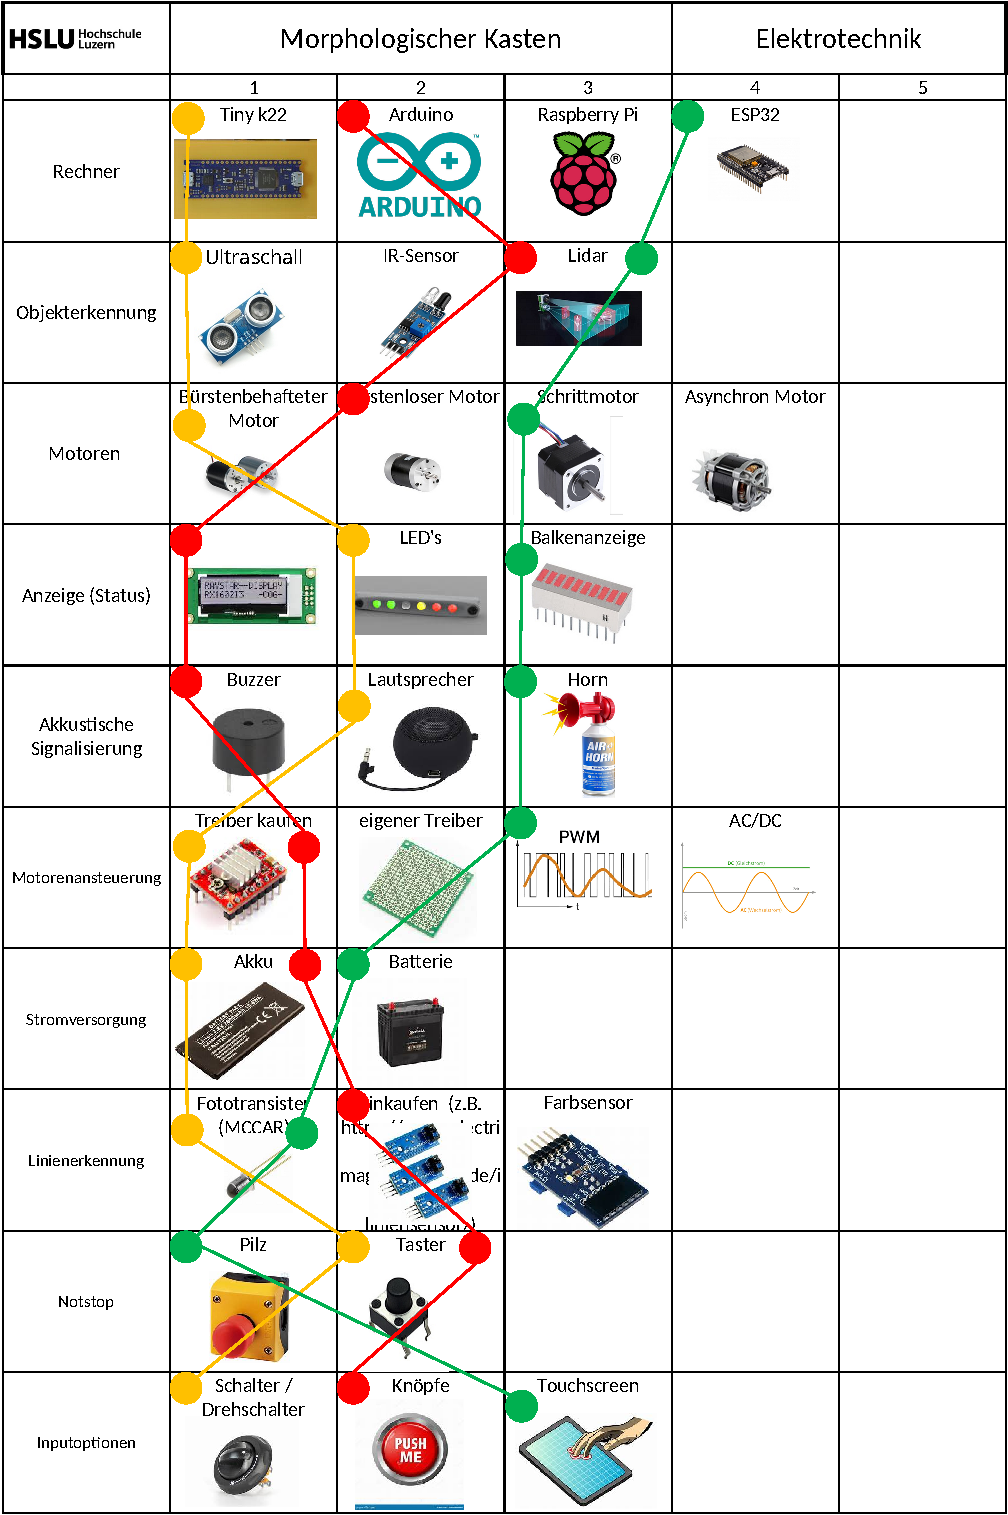
\includegraphics[height=\textheight-1cm]{assets/MK_Elektrotechnik.pdf}
%\caption{Morphologischer Kasten: Elektrotechnik}
%\label{table:MK-Elektrotechnik}
%\end{table}
%\newpage
%\begin{table}[H]
%\centering
%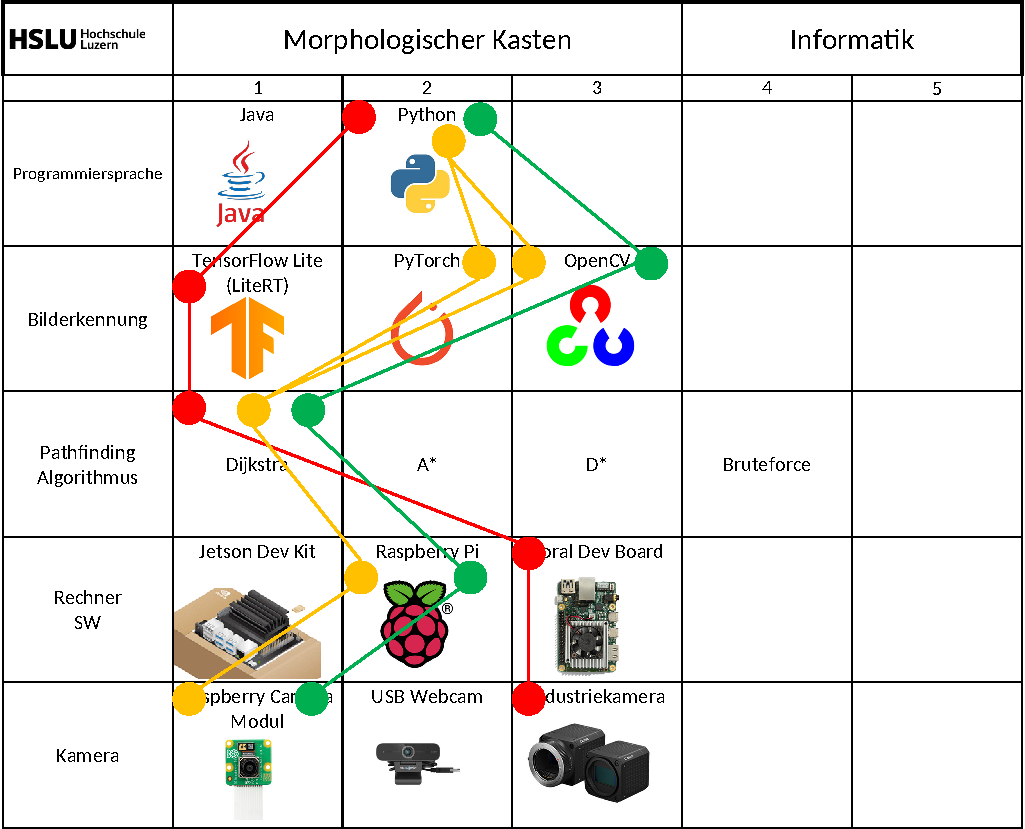
\includegraphics[width=\textwidth]{assets/MK_Informatik.pdf}
%\caption{Morphologischer Kasten: Informatik}
%\label{table:MK-Informatik}
%\end{table}
%\newpage
%\begin{table}[H]
%\centering
%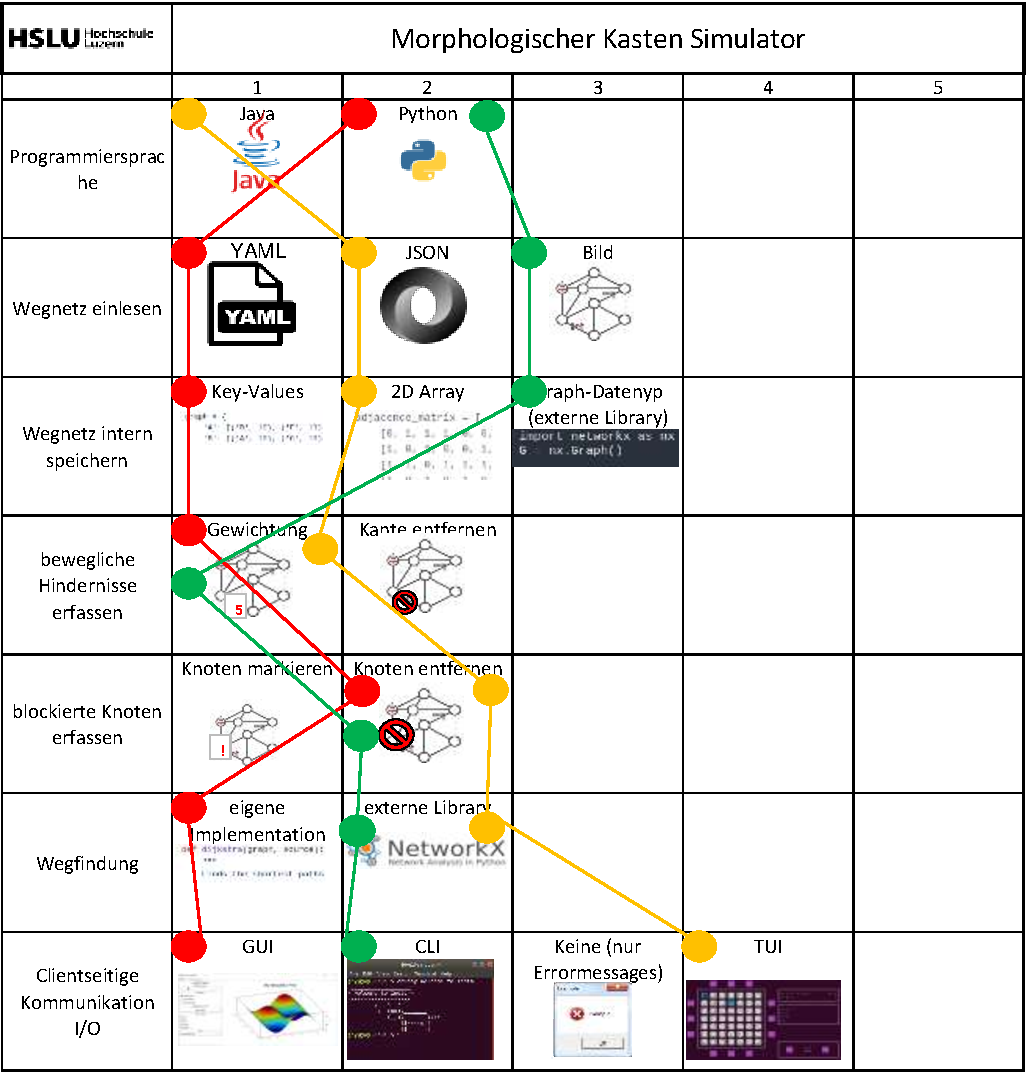
\includegraphics[width=\textwidth]{assets/MK_Simulator.pdf}
%\caption{Morphologischer Kasten: Simulator}
%\label{table:MK-Simulator}
%\end{table}
%\newpage


%%% THIS IS USELESS %%%%%%%%%%%%

% \subsection{Originale Aufgabenstellung}\label{aufgabenstellung}

% Nachfolgend ist die originale Aufgabenstellung angehängt.

% 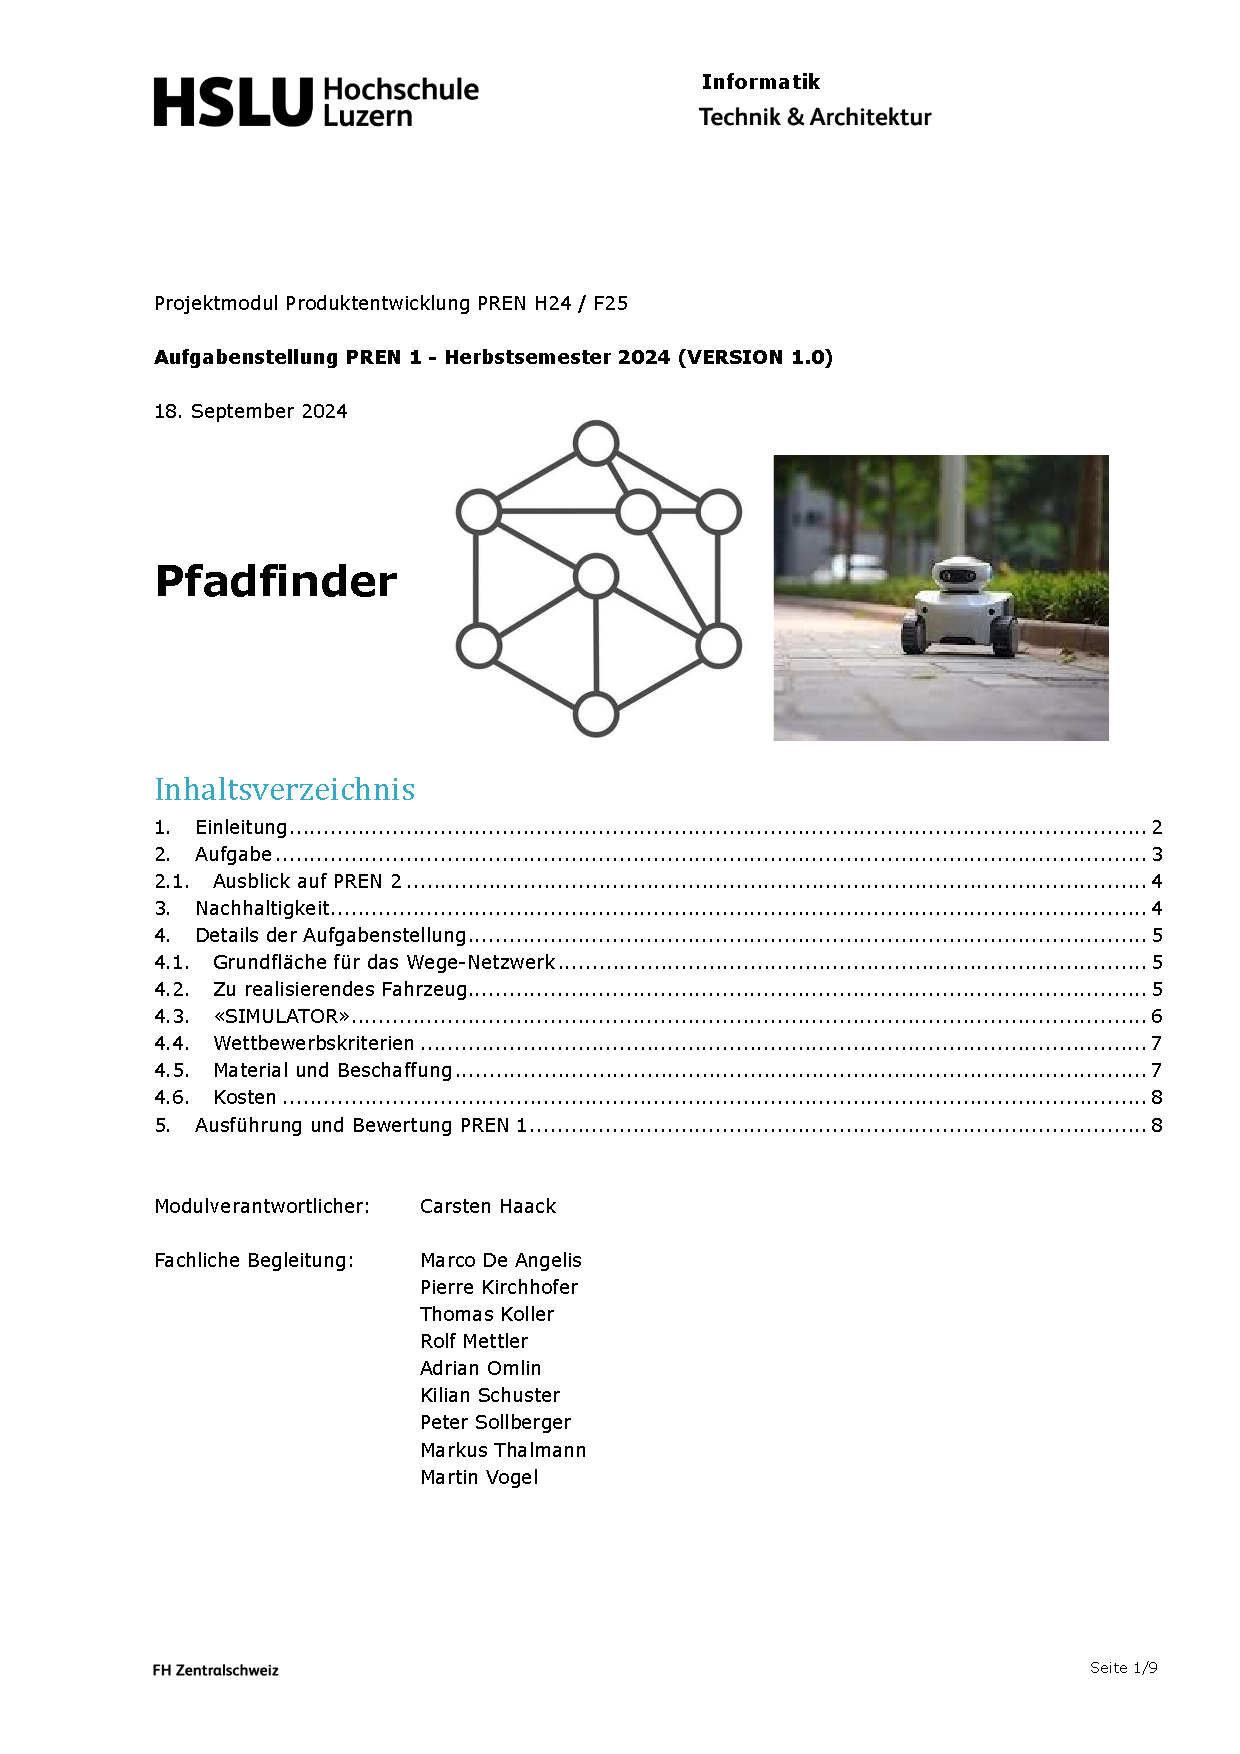
\includepdf[pages=-]{assets/AufgabenstellungPREN1HS24.pdf}



\end{document}